% This is samplepaper.tex, a sample chapter demonstrating the
% LLNCS macro package for Springer Computer Science proceedings;
% Version 2.20 of 2017/10/04
%
\documentclass[runningheads]{llncs}
%
\usepackage{graphicx}
\usepackage{hyperref}
\usepackage{amsmath}
\usepackage{tabularx}
\usepackage{ragged2e,booktabs,caption}
\usepackage{amsfonts}
\usepackage{amssymb}
\usepackage{listings}
\usepackage{algorithm}
\usepackage{algpseudocode}
% Used for displaying a sample figure. If possible, figure files should
% be included in EPS format.
%
% If you use the hyperref package, please uncomment the following line
% to display URLs in blue roman font according to Springer's eBook style:
% \renewcommand\UrlFont{\color{blue}\rmfamily}
\lstset{
  basicstyle=\ttfamily,
  columns=fullflexible,
  showstringspaces=false,
  commentstyle=\color{gray}\upshape
}

\lstdefinelanguage{XML}
{
  morestring=[b]",
  morestring=[s]{>}{<},
  morecomment=[s]{<?}{?>},
  stringstyle=\color{black},
  identifierstyle=\color{darkblue},
  keywordstyle=\color{cyan},
  morekeywords={xmlns=,version,type,
  Tr}% list your attributes here
}
\begin{document}
%
\title{Mersul Trenurilor\thanks{Project proposed by Continental} - a proposed concurrent server}
%
%\titlerunning{Abbreviated paper title}
% If the paper title is too long for the running head, you can set
% an abbreviated paper title here
%
\author{Tudor Ilade}
%
% First names are abbreviated in the running head.
% If there are more than two authors, 'et al.' is used.
%
\institute{Department of Computer Science, "Alexandru Ioan Cuza" University, Iasi
\vspace{0.5mm}
\email{tudor.ilade@yahoo.com}}
%
\maketitle              % typeset the header of the contribution
%
\begin{abstract}
This paper proposes a design of a concurrent server for the project "Mersul Trenurilor". The projects consists on implementing a basic network protocol that contains a server which will concurrently handle various type of requests from multiple clients. The communication client-server will be implemented using TCP/IP protocol.

\keywords{Mersul Trenurilor  \and Network \and TCP/IP protocol.}
\end{abstract}
%
%
%
\section{Introduction}
I choose this project because it seems to me that it has an important practical application and I am interested to see what problems can arose during its development and how should I tackle efficiently design problems.

In this paper I will propose an application design of "Mersul Trenurilor" project using network communication. The main focus will be on developing a scalable and concurrent architecture of the server. 

\section{Technologies}
\subsection{TCP/IP Protocol}
The project will use as client-server communication protocol the TCP/IP. I am interested to implement a reliable, straightforward way to exchange data without having to worry about lost packets or jumbled data. This feature is important because clients cannot only read information from server, but also can modify existing data from a XML file.

When a client sends a request to the server that modifies data, I want to be sure that the data arrives at server is correct and complete and it is updated accordingly. The integrity and accuracy of data is important, otherwise clients who just want to know when next train leaves, might loose the train because of an incorrect update from a previous request. 

Thus, I find TCP/IP protocol the best fit for this project \cite{ref_url1} because is reliable, connection-oriented and full-duplex. The three-way-shake algorithm facilitates the connection between server and client and guarantees data transmission without any loss.

\subsection{Qt SDK}
I aim to wrap the client-server communication around a GUI implemented with the help of Qt SDK for C++.

\subsection{Qt XML C++}
The application will perform Read/Write operations from/to an XML file. This operations will be implemented with the help of Qt XML C++ Classes module. \cite{ref_url3}

\section{Architecture}

The architecture of application is presented in the following diagram:

\subsection{Server}
\hspace*{-1.2in}
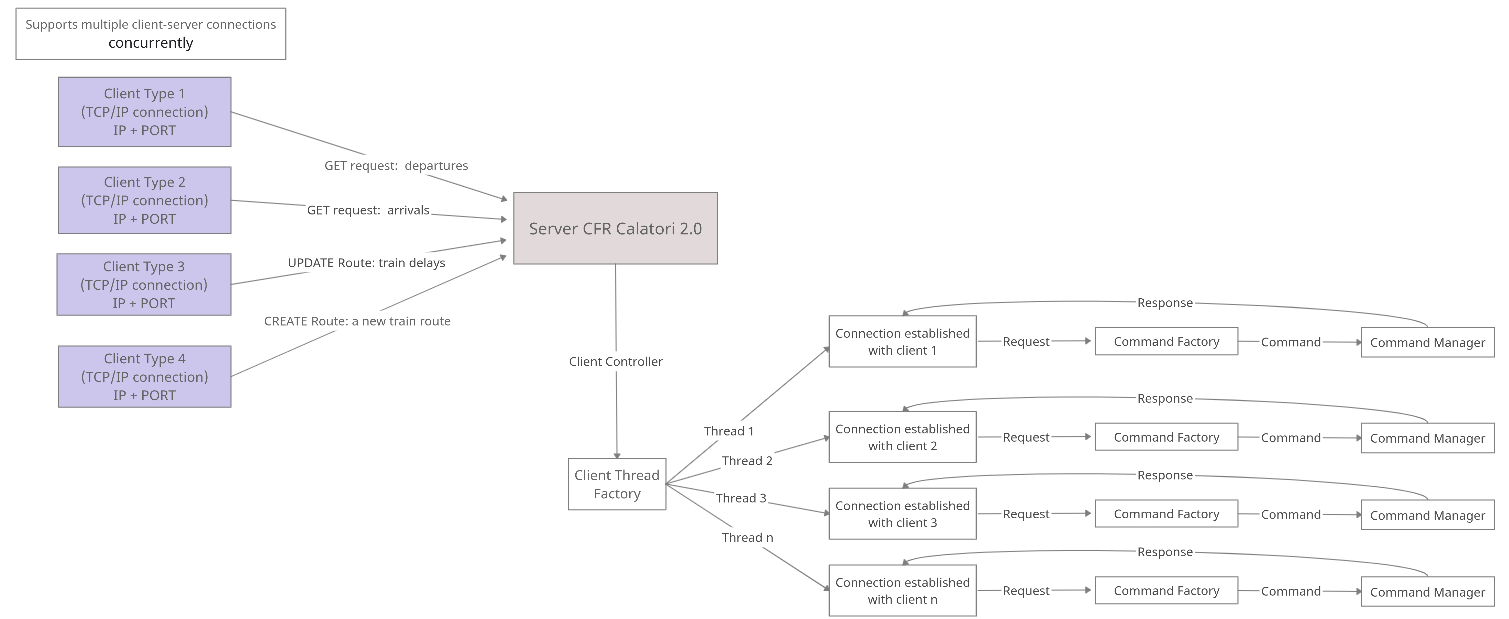
\includegraphics[scale=0.34]{retele4.png}


The application will support two classes of commands:

$\rightarrow$ Retrieving data

$\rightarrow$ Manipulating data

Retrieving data commands will consist in GET requests, as follows:

\begin{enumerate}
    \item Client type 1 $\rightarrow$ GET DEPARTURES: Any connected client can ask for information about departures of trains in the current day.
    \item Client type 2 $\rightarrow$ GET ARRIVALS: Any connected client can ask for information about arrivals of trains from the following hour or current day or for a given train if ID is provided.
\end{enumerate}

 For GET ARRIVALS/DEPARTURES commands, I will implement two flags: $-hour$ and $-id <train\_id>$. $-hour$ flag will ask for arrivals/departures in the next hour. $<train\_id>$ will ask for arrivals/departures of the given train id, in the given day. A combination of both will result in geting the arrivals/departures of the given train id in the next hour. If any delays are present at the request time, will be reflected in the result message with estimated time of arrival/departure.


\begin{enumerate}
    \item Client type 3 $\rightarrow$ UPDATE ROUTE: Any connected client can modify the schedule details of a train by providing delay time in minutes.
    \item Client type 4 $\rightarrow$ CREATE request: A client with CREATE permissions will be able to add a new route.
\end{enumerate}

UPDATE ROUTE and CREATE ROUTE commands will have the format:  $$ \rightarrow \textbf{UPDATE ROUTE} \;\; <train\_id> \; <delay\_time>.
$$
$$ \rightarrow \textbf{CREATE ROUTE} <train\_id>$$

CREATE ROUTE command will check first for the provided train id whether exists in XML file. If it doesn't, then a dashboard will appear where he or she will have to insert the following details, comma separated:

    $\rightarrow$ $station_1$-$departs$-$arrival$-$delay$, \cdots, $station_n$-$departs$-$arrival$-$delay$

\subsection{Client}
The client architecture looks as follow:

\vspace{5mm}
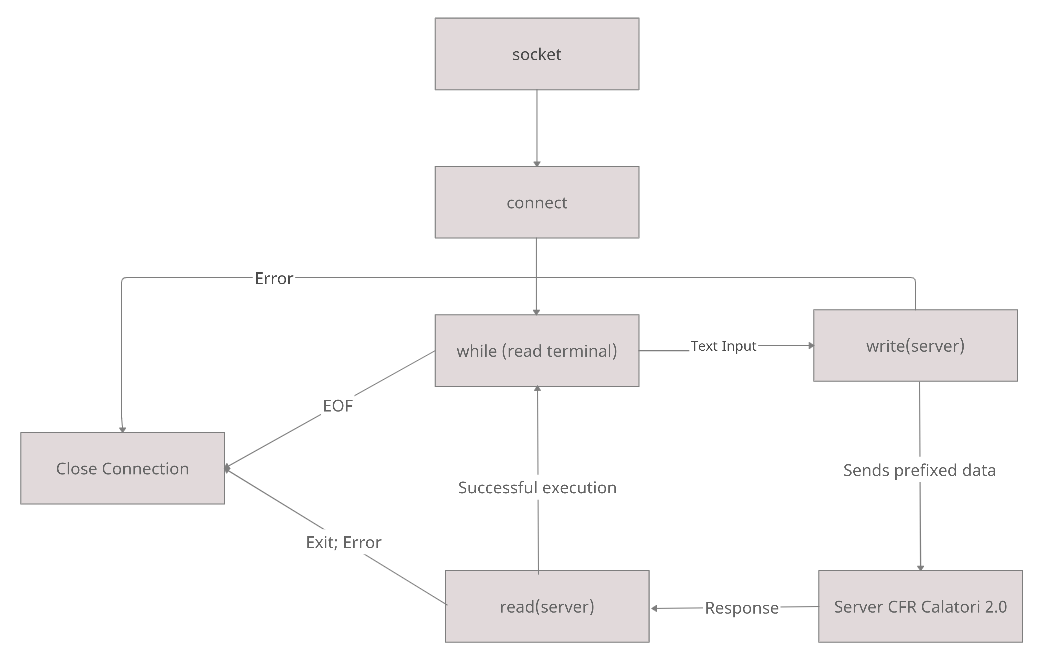
\includegraphics[scale=0.35]{client.png}
\vspace{5mm}

\section{Implementation}

All clients will be served concurrently. The mechanism to serve clients in parallel will be based on multithreading.
This mechanism will be implemented with the help of a factory design pattern called Client Thread Factory. Clients will be served to Client Thread Factory by a Client Controller.

The Client Controller will be a class that will have the main responsability of listening and serving new clients, once the connection is successfully established, to Client Thread Factory class.

The Client Thread Factory design pattern will be responsible with the handling of new connection requests. The problem with handling multiple connection requests at the same time will be tackled with a prethreading protection mechanism that will serve requests once at a time and send descriptors to the next empty slot from threading pool. This will be achieved with the help of \textbf{Accept} primitive.

The aforementioned design patterns are implemented as follows:

\vspace{5mm}

\hspace*{-0.3in}
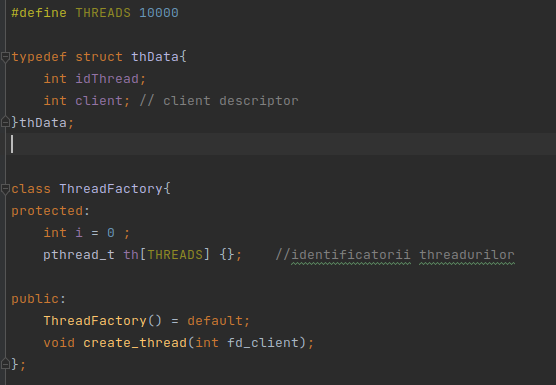
\includegraphics[scale=0.35]{thread_factory.png}
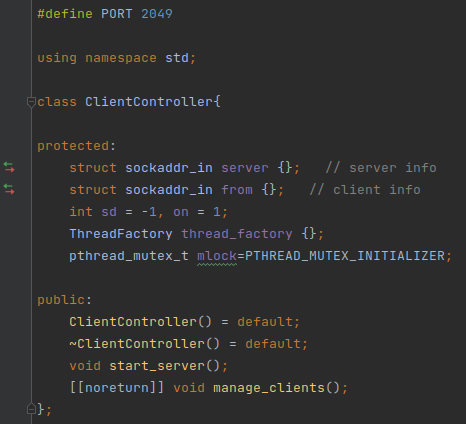
\includegraphics[scale=0.35]{client_Controller.png}

\vspace{5mm}



After client is successfully connected to server, it will receive a success message from server. At this phase, clients can now send requests to server. All the requests will be handled by a Request Controller Its main responsabilities will be:


\begin{enumerate}
    \item Receive request
    \item Send the request to Command Factory and convert it to corresponding Command
    \item Handle the Command to Command Manager
    \item Queue the command
\end{enumerate}

Requests are transformed into the corresponding command by CommandFactory class. Commands are implemented with the help of a Command abstract class that is inherited by all available commands. The command will store all the relevant info needed for processing, such as client descriptor, CommandResult. Once the command has been transformed, will be parsed to Command Manager to queue it.


\vspace{5mm}

\hspace*{-1.3in}
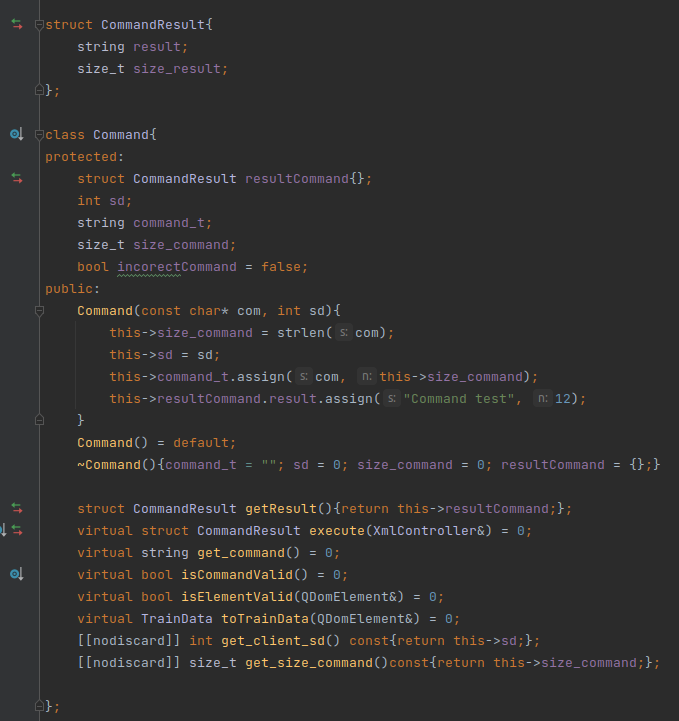
\includegraphics[scale=0.3]{commandABC.png}
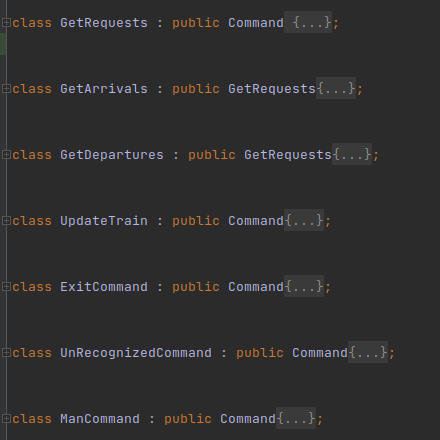
\includegraphics[scale=0.3]{commands.png}
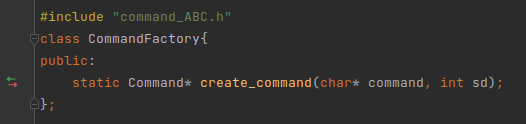
\includegraphics[scale=0.3]{cmd_Factory.png}

\vspace{5mm}

The Command Manager implements a Command Queue where requests will be stored and served according to LIFO rule. The Command Manager has is  own threading pool from where it constantly checks the queue. If any command will be add, will be popped from top of the queue and sent to execution. Once the result is obtained, it will send the response to the client. After a client is served, the Command Manager will look at Command Queue and send to processing the next command.

\vspace{1.5mm}
\hspace{+1in}
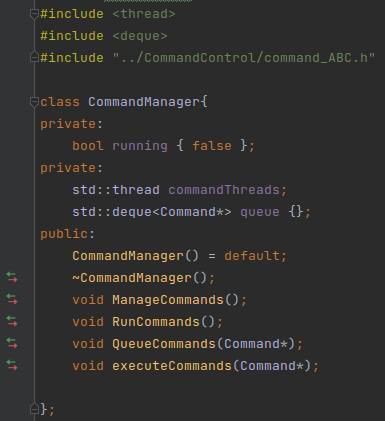
\includegraphics[scale=0.5]{command_manager.png}
\vspace{1.5mm}

The communication between client and server are in both way prefixed with the length of data ready to be sent. The prefixed communication consists in writing the size of data as integer at the beginning of each message, followed by data.


The mechanism of reading/writing the XML file will be done concurrently. In the implementation, will be used a locks to prevent data race condition.\cite{ref_url2} Each client will read the data is available at the time of processing. For the write requests, the critical section will be protected with the help of flock struct from fcntl header.

The XML file will have the following structure:

\begin{lstlisting}
<?xml version="1.0" encoding="utf-8"?>
<xs:schema attributeFormDefault="unqualified" elementFormDefault="qualified"
   xmlns:xs="http://www.w3.org/2001/XMLSchema">
  <Trains>
    <Train>
        <id>Train Id<\id>
        <stations>
            <station id=1 departs=14:01 arrives=0 delay=0>Ramnicu Valcea<\station>
            <station id=2 arrives=14:34 departs=14:36 delay=0 >Pitesti<\station>
            <station id=3 departs=0 arrives=16:01 delay=10 >Bucuresti Nord<\station>
        <\stations>
    </Train>
    
    <Train>
        <id>Train Id<\id>
        <stations>
            <station id=1 departs=06:21 arrives=0 delay=10>Iasi<\station>
            <station id=2 arrives=08:43 departs=08:44 delay=12 >Focsani<\station>
            <station id=3 departs=0 arrives=14:55 delay=7 >Bucuresti Nord<\station>
        <\stations>
    </Train>

    ...

    <Train>
        <id>Train Id<\id>
        <stations>
            <station id=1 departs=02:01 arrives=0 delay=0>Cluj-Napoca<\station>
            <station id=2 arrives=03:23 departs=03:30 delay=0 >Sighisoara<\station>
            <station id=3 departs=0 arrives=06:42 delay=10 >Brasov<\station>
        <\stations>
    </Train>
  </Trains>
</xs:schema>
\end{lstlisting}




\section{Conclusion}

This was my proposed implementation of the Mersul Trenurilor project. Further improvements can be done by adding more features to it. Some possible features that can be added are:

$\rightarrow$ The possibility of client to choose the type of connection they want (TCP/IP or UDP) for GET requests. In this case, usually the client wants to know fast some details about a train. In majority of cases this protocol will yield the desired result without data loss. And even so, the Client can send another request if he or she sees that nothing has been returned. The majority of requests of this server will be of type GET, rather than PUT or CREATE. Thus, the feature can result into much faster exchange of information.

$\rightarrow$ A backup mechanism implemented for XML file to make sure that in case of failures, data is backed up periodically and prevents massive data loss.

$\rightarrow$ A secured connection by providing a TOKEN in case of writing data on XML. The TOKEN can be generated uniquely in UUID4 format, thus only trusted users can perform Write operations.


\begin{thebibliography}{8}

\bibitem{ref_book1}
W. Richard Stevens, Bill Fenner, Andrew M. Rudoff,
UNIX Network Programming Volume 1, Third Edition: The Sockets Networking API, 3rd. ed. Publisher,
Addison Wesley (2003)
\bibitem{ref_url1}
Computer Networks Homepage, \url{https://profs.info.uaic.ro/~computernetworks/index.php}. Last accessed 1 dec 2022
\bibitem{ref_url2}
Mutex lock for threads, \url{https://www.geeksforgeeks.org/mutex-lock-for-linux-thread-synchronization/}. Last accessed 1 dec 2022
\bibitem{ref_url3}
Qt XML docpage, \url{https://doc.qt.io/qt-6/qtxml-module.html}. Last accessed 1 dec 2022
\end{thebibliography}
\end{document}
